\chapter{HPX-RTE}
\label{sec:HPX-RTE}

ParalleX and HPX are both parts of the eXascale Programming Environment and System Software (XPRESS)~\cite{huck2013early,brightwell2013xpress} project funded by the Department of Energy.

The goals of XPRESS project are:
\begin{itemize}
\item ``Enable exascale performance capability for current and future Department of Energy applications
\item Develop and deliver a practical computing system software X‐stack, “OpenX”, for future practical DOE computing systems
\item Provide programming methods, environments, languages, and tools for effective means of expressing application and system software for portable exascale system execution''~\cite{xpress}
\end{itemize}

This project is a collaboration between Sandia National Laboratories (SNL), Indiana University (IU), Lawrence Berkeley National Laboratory (LBNL), Louisiana State University (LSU), Oak Ridge National Laboratory (ORNL), University of Houston (UH), University of North Carolina at Chapel Hill/RENCI (UNC/RENCI), and University of Oregon (UO).


\begin{figure}[h!]
\centering
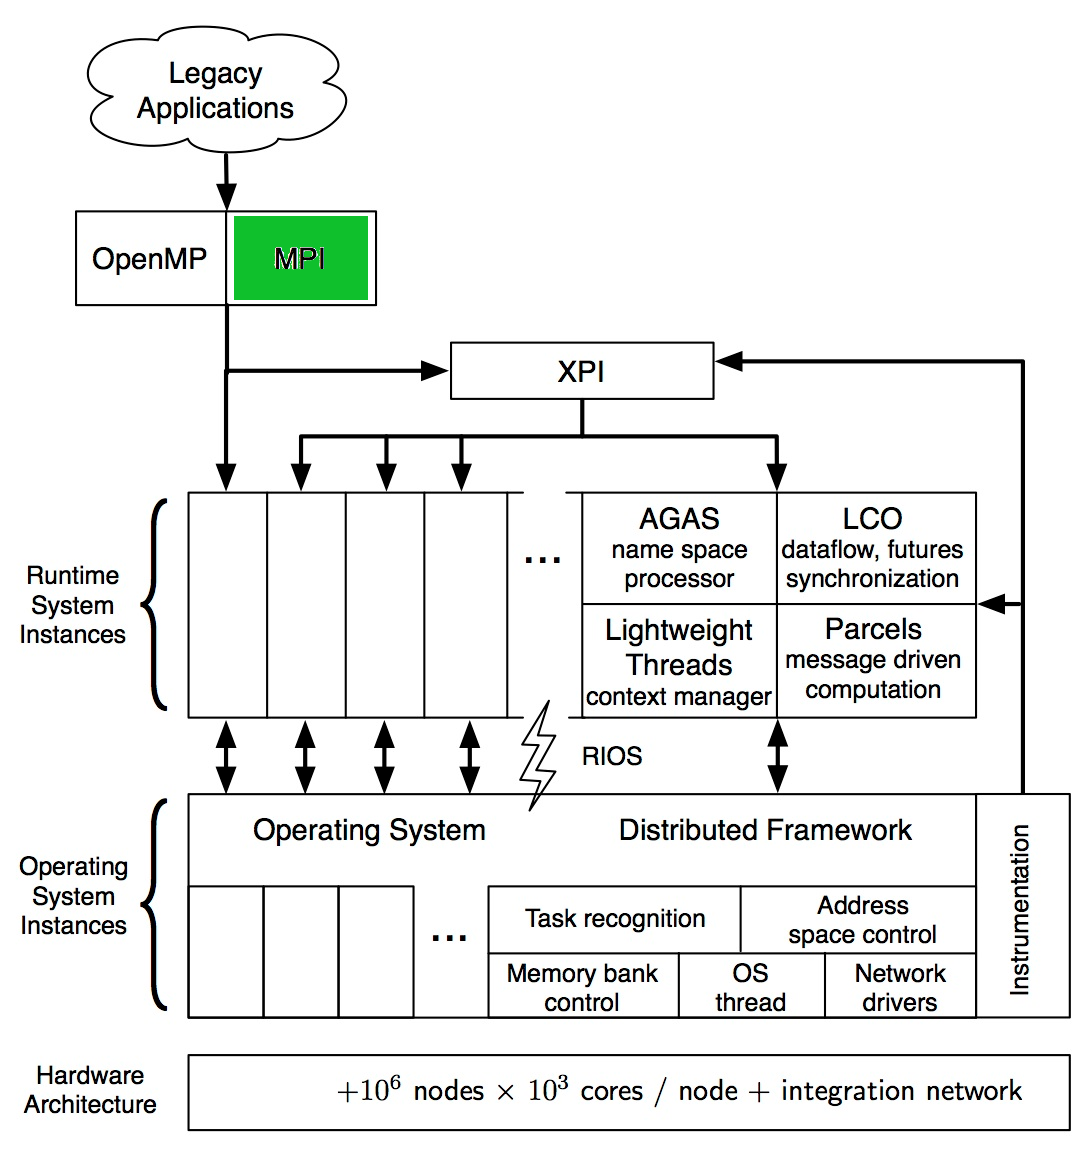
\includegraphics[scale=0.8]{images/openx.png}
\caption[The OpenX Software Architecture]{The OpenX Software Architecture}
\label{fig:openx}
\end{figure}


\section{Design Principles}
\label{sec:design}

\begin{itemize}
\item \textbf{Functionality}\\
  s
\item \textbf{Simplicity}\\
  s
\item \textbf{Code reuse}\\
  s
\item \textbf{Modularity}\\
s
\end{itemize}

\begin{figure}[h!]
\centering
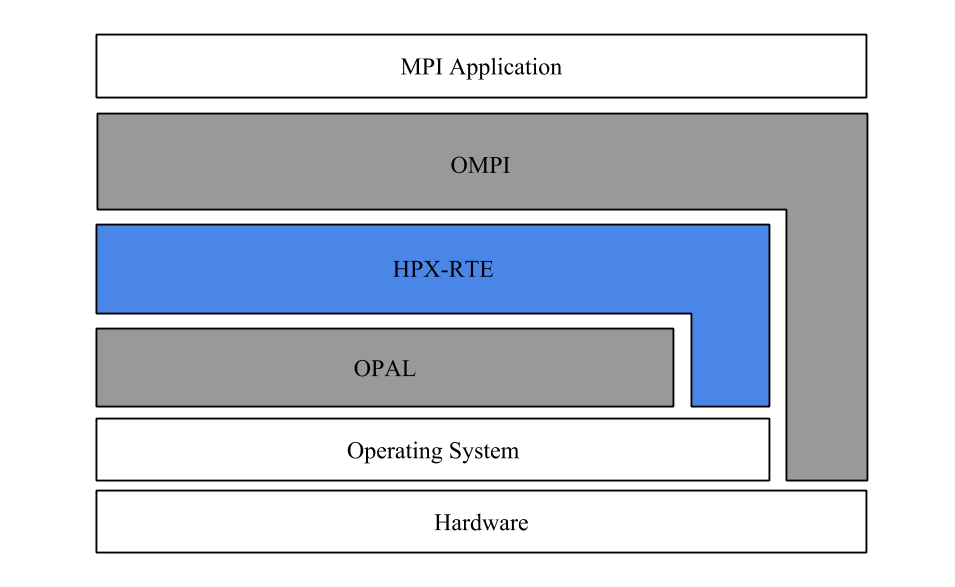
\includegraphics[scale=0.4]{images/open-mpi-layers-hpx-rte.png}
\caption[Open MPI Layers using HPX-RTE]{Open MPI Layers using HPX-RTE}
\label{fig:open-mpi-layers-hpx-rte}
\end{figure}

\section{Challenges}
\label{sec:challenges}

\subsection{C and C++}
\subsection{Imperfect Abstraction in ORTE}
\subsection{Fundamental Differences}

\section{Architecture}
\label{sec:architecture}

\iffalse
 This is the public RTE interface to the OMPI layer. Any RTE can be
 connected to the OMPI layer by creating a new static component in
 this framework, assigning it a priority and including a configure.m4
 to define when it should be built.

 Each component must provide a number of types and functions that mimic
 those provided by ORTE. These include (where flexibility exists, the
 ORTE data type is shown, but any compatible type is allowed. For example,
 the jobid field in ompi_process_name_t could be any type of integer, but
 cannot be a string):

 (a) Process name objects and operations
     1. Definitions for integral types ompi_jobid_t and ompi_vpid_t.
        The jobid must be unique for a given MPI_COMM_WORLD capable of
        connecting to another OMPI_COMM_WORLD and the vpid will be the
        process's rank in MPI_COMM_WORLD.
     2. ompi_process_name_t - a struct that must contain at least two integer-typed fields:
           a. ompi_jobid_t jobid
           b. ompi_vpid_t vpid
        Note that the structure can contain any number of fields beyond these
        two, so the process name struct for any particular RTE can be whatever
        is desired.
     3. OMPI_NAME_PRINT - a macro that prints a process name when given
        a pointer to ompi_process_name_t. The output format is to be
        a single string representing the name.  This function should
        be thread-safe for multiple threads to call simultaneously.
     4. OMPI_PROC_MY_NAME - a pointer to a global variable containing
        the ompi_process_name_t for this process. Typically, this is
        stored as a field in the ompi_process_info_t struct, but that
        is not a requirement.
     5. OMPI_NAME_WIlDCARD - a wildcard name.
     6. ompi_rte_compare_name_fields - a function used to compare fields
        in the ompi_process_name_t struct. The function prototype must be
        of the form:
        int ompi_rte_compare_name_fields(ompi_rte_cmp_bitmask_t mask,
                                         ompi_process_name_t *name1,
                                         ompi_process_name_t *name2);
        The bitmask must be defined to indicate the fields to be used
        in the comparison. Fields not included in the mask must be ignored.
        Supported bitmask values must include:
           b. OMPI_RTE_CMP_JOBID
           c. OMPI_RTE_CMP_VPID
           d. OMPI_RTE_CMP_ALL
      7. uint64_t ompi_rte_hash_name(name) - return a string hash uniquely
         representing the ompi_process_name passed in.
      8. OMPI_NAME - an Opal DSS constant for a handler already registered
         to serialize/deserialize an ompi_process_name_t structure.

 (b) Collective objects and operations
     1. ompi_rte_collective_t - an OPAL object used during RTE collective operations
        such as modex and barrier. It must be an opal_list_item_t and contain the
        following fields:
           a. id (ORTE type: int32_t)
           b. bool active
              flag that user can poll on to know when collective
              has completed - set to false just prior to
              calling user callback function, if provided
     2. ompi_rte_modex - a function that performs an exchange of endpoint information
        to wireup the MPI transports. The function prototype must be of the form:
        int ompi_rte_modex(ompi_rte_collective_t *coll);
        At the completion of the modex operation, the coll->active flag must be set
        to false, and the endpoint information must be stored in the modex database.
        This function must have barrier semantics across the MPI_COMM_WORLD of the
        calling process.
     3. ompi_rte_barrier - a function that performs a barrier operation within the
        RTE. The function prototype must be of the form:
        int ompi_rte_barrier(ompi_rte_collective_t *coll);
        At the completion of the barrier operation, the coll->active flag must be set
        to false

 (c) Process info struct
     1. ompi_process_info_t - a struct containing info about the current process.
        The struct must contain at least the following fields:
           a. app_num -
           b. pid - this process's pid.  Should be same as getpid().
           c. num_procs - Number of processes in this job (ie, MCW)
           d. my_node_rank - relative rank on local node to other peers this run-time
                    instance knows about.  If doing dynamics, this may be something
                    different than my_local_rank, but will be my_local_rank in a
                    static job.
           d. my_local_rank - relative rank on local node with other peers in this job (ie, MCW)
           e. num_local_peers - Number of local peers (peers in MCW on your node)
           f. my_hnp_uri -
           g. peer_modex - a collective id for the modex operation
           h. peer_init_barrier - a collective id for the barrier during MPI_Init
           i. peer_fini_barrier - a collective id for the barrier during MPI_Finalize
           j. job_session_dir -
           k. proc_session_dir -
           l. nodename - a string representation for the name of the node this
              process is on
           m. cpuset -
     2. ompi_process_info - a global instance of the ompi_process_t structure.
     3. ompi_rte_proc_is_bound - global boolean that will be true if the runtime bound
        the process to a particular core or set of cores and is false otherwise.

 (d) Error handling objects and operations
     1. void ompi_rte_abort(int err_code, char *fmt, ...) - Abort the current
        process with the specified error code and message.
     2. int ompi_rte_abort_peers(ompi_process_name_t *procs, size_t nprocs) -
        Abort the specified list of peers
     3. OMPI_ERROR_LOG(rc) - print error message regarding the given return code
     4. ompi_rte_register_errhandler - register a callback function for the RTE
        to report asynchronous errors to the caller

 (e) Init and finalize objects and operations
     1. ompi_rte_init - a function to initialize the RTE. The function
        prototype must be of the form:
        int ompi_rte_init(int *argc, char ***argv);
     2. ompi_rte_finalize - a function to finalize the RTE. The function
        prototype must be of the form:
        int ompi_rte_finalize(void);
     3. void ompi_rte_wait_for_debugger(void) - Called during MPI_Init, this
        function is used to wait for debuggers to do their pre-MPI attach.
        If there is no attached debugger, this function will not block.

 (f) Database operations
     1. ompi_rte_db_store - a function to store modex and other data in
        a local database. The function is primarily used for storing modex
        data, but can be used for general purposes. The prototype must be
        of the form:
        int ompi_rte_db_store(const ompi_process_name_t *proc,
                              const char *key, const void *data,
                              opal_data_type_t type);
        The implementation of this function must store a COPY of the data
        provided - the data is NOT guaranteed to be valid after return
        from the call.
     3. ompi_rte_db_fetch -
        NOTE: Fetch accepts an 'ompi_proc_t'.
        int ompi_rte_db_fetch(const struct ompi_proc_t *proc,
                              const char *key,
                              void **data,
                              opal_data_type_t type);
     4. ompi_rte_db_fetch_pointer -
        NOTE: Fetch accepts an 'ompi_proc_t'.
        int ompi_rte_db_fetch_pointer(const struct ompi_proc_t *proc,
                                      const char *key,
                                      void **data,
                                      opal_data_type_t type);
     5. Pre-defined db keys (with associated values after rte_init)
        a. OMPI_DB_HOSTNAME
        b. OMPI_DB_LOCALITY

  (g) Communication support

\fi

\section{Implementation}
\label{sec:implementation}
MPI system level adjustment, and change of configuration logic

\iffalse

what we have done?
Open MPI has an abstraction layer for runtime environments.
We provide that abstraction layer using hpx.
The abstraction is imperfect(lack of documentation,
not perfect interface independences)
Key components we had to develop?
- distributed key-value store and fetch using hpx actions
- barrier (synchronization point) using hpx actions
- translation table from hpx localities to mpi ranks
- populating some internal data structures
- extract and populate some key-value pairs into the db:
some are set in orte layer and used in ompi layer
- hacking the configure logic to detect and handle boost and HPX libraries
and modify the generated make files accordingly
- using c++ to compile a number of components
- manually exclude some components that are deeply entangled with rte
- intercepting printf from c code to see the output


current status:
- hpx 0.9.9
- openmpi 1.8.4
- restrctions: - one rank per locality
- launch with ssh
- communication protocols:
tcp: - tests (including communication) are running now
shared memory: -not tried recently, it did not work early on

questions/topics to discuss:
- os functionalities and interactio with hpx: fork, pipe, mmap
- slurm integration

\fi
